\section{Анализ предметной области}


\subsection{Анализ методов автоматического создания расписания учебных занятий}

Задача создания расписания сводится к формированию и оптимизации процесса обслуживания конечного множества требований (заявок) на осуществление действий в системе. Задача составления расписания учебного заведения относится к классу NP-hard задач, она сводится к распределению трёх ресурсов: преподавательского состава, студенческого состава и аудиторий учебного заведения. Детальная постановка задачи, требования к расписанию и предлагаемый алгоритм приводятся во второй главе? в настоящей главе рассматриваются существующие методы решения и обосновывается выбор гибридного подхода.

Если посмотреть на количество научных статей (см. \figref{fig:relevance}), публикуемых международным сообществом на эту тему за последние пару десятков лет \cite{vrielink:patat2016}, то можно сделать вывод, что область образовательной логистики всё ещё является актуальной темой исследований и разработки.

\begin{figure}[H]
	\centering
	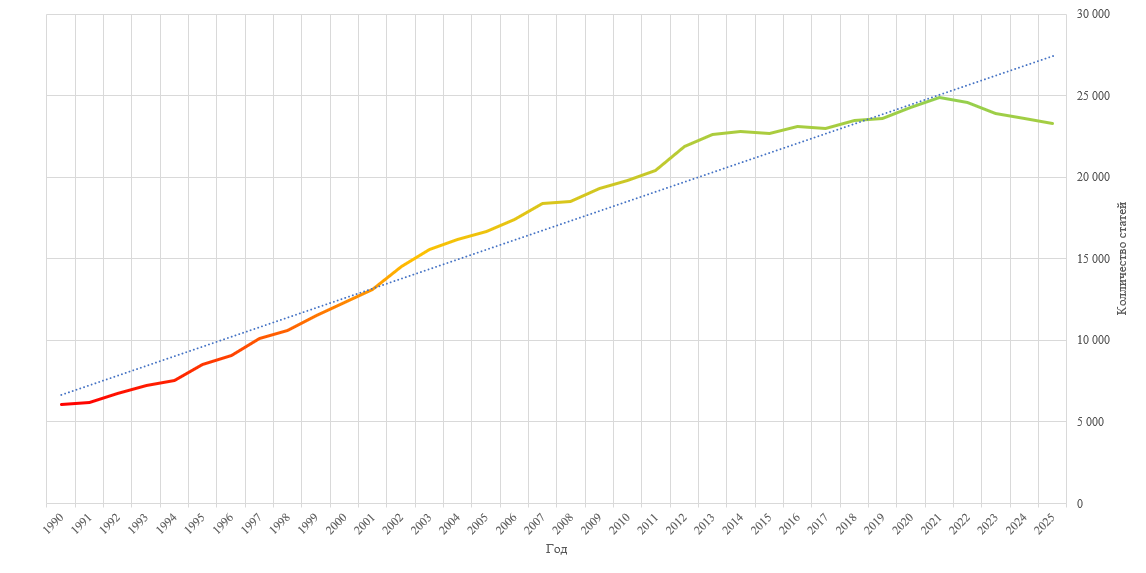
\includegraphics[width=1\textwidth]{images/ch1/relevance.png}
	\caption{Количество статей по годам на тему расписаний в высших учебных заведениях в Google Scholar по поисковому запросу «(timetabling OR timetable) AND higher education»}
	\label{fig:relevance}
\end{figure}

Для того, чтобы разобраться на каком этапе сейчас эта область, стоит проанализировать различные подходы и выявить основные тенденции и идеи.

\subsubsection{Линейные и целочисленные программные методы составления расписания}

Одними из первых, кто предоставил стратегии раскраски графов для решения проблемы составления расписания были Уэлш и Пауэлл (1967) \cite{welsh:chromatic}. Они заложили основу для более сложных исследований графовых эвристик в составлении расписания \cite{merlot:hybrid}. Эвристики составления расписания на основе раскраски графов - это полезный метод, на котором строится их оценка и улучшение.

Линейные и целочисленные программные методы - это математические алгоритмы, которые присваивают целочисленные значения переменным. Вариации этого метода были и до сих пор широко используются для решения комбинаторных задач оптимизации. Эти методы включают в себя программирование с ограничениями и методы удовлетворения ограничений.

Однако такие методы, как правило, требуют больших вычислительных ресурсов из-за экспоненциального количества переменных.

\subsubsection{Метаэвристики}

Метаэвристика --- это метод оптимизации, многократно использующий простые правила или эвристики для достижения оптимального или субоптимального решения. С 1995 по 2010 годы методологические подходы к решению проблем составления расписания обычно классифицировались на две категории метаэвристик: популяционные и одиночные \cite{burke:timepredefined}. Если классифицировать основные подходы и алгоритмы, то можно построить следующий график (см. \figref{fig:metaheuristics}).

\begin{figure}[H]
	\centering
	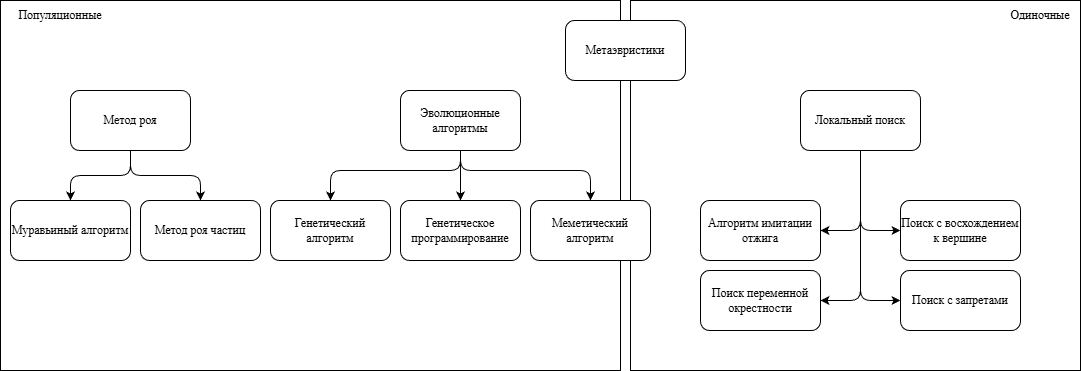
\includegraphics[width=1\textwidth]{images/ch1/metaheuristics.png}
	\caption{Классификация алгоритмов решения задачи}
	\label{fig:metaheuristics}
\end{figure}

Метаэвристический подход позволяет быстро получить приемлемое решение популяционным алгоритмом, а впоследствии улучшать его и удовлетворять дополнительные ограничения итеративным образом с помощью одиночных методов локального поиска.

Естественно нет возможности окунуться с деталями в каждый подход, но стоит хотя бы поверхностно изучить и оценить разные метаэвристические методы.

\paragraph{Локальные алгоритмы}

\subparagraph{Поиск с запретами.}

Поиск с запретами (Tabu search) относится к методологиям локального поиска и основан на поиске градиентного спуска. Существует несколько актуальных работ, в которых проведено ценное исследование методов поиска с запретами \cite{digaspero:tabu,petrovic:trajectories}. Исследования основаны на диверсификации соседей, при котором поиск расширяется для нахождения большего количества локальных оптимумов. Это приводит к интенсификации шагов и более быстрого нахождения решения.

Однако поиск с запретами имеет тенденцию застрять в подоптимальных областях или плато. Подоптимальные области - это регионы пространства поиска, где текущее решение локально оптимально, но не обязательно глобально. Плато представляют собой плоские области функции, где градиент близок к нулю, что затрудняет продвижение поиска.

\subparagraph{Алгоритм имитации отжига.}

Алгоритм SA --- это ещё один метод локального поиска. SA вдохновлён физическим процессом отжига металла, при котором нагреваемый металл постепенно остывает, обеспечивая более устойчивую кристаллическую структуру. В контексте оптимизации, этот метод направлен на поиск более широкой области пространства поиска, в которой принимаются худшие шаги и допускается более широкий поиск оптимального решения. Существует множество вариаций SA \cite{burke:timepredefined,dowsland:simulatedannealing}, он часто комбинируется с алгоритмом восхождения к вершине \cite{qu:survey}, или программированием с ограничениями \cite{brailsford:csp}.

Идеи стохастического локального поиска, заложенные в SA, используются в предлагаемом алгоритме на этапе оптимизации расписания при реализации repair-мутаций и локального поиска по целевой функции.

\paragraph{Эволюционные алгоритмы}

\subparagraph{Генетические алгоритмы.}

Среди эволюционных алгоритмов одними из самых изученных и популярных являются генетические алгоритмы (Genetic algorithms) \cite{corne:evolutionary}. Эти алгоритмы моделируют процесс естественного отбора, таким образом находя более совершенную форму «жизни».

\subparagraph{Меметические алгоритмы.}

Как дополнение к генетическим алгоритмам рассматриваются меметические алгоритмы \cite{burke:memetic}. Меметические алгоритмы (Memetic algorithms) представляют собой эволюционный метод оптимизации, который объединяет генетические алгоритмы с понятием «мема» из теории эволюции Ричарда Докинза. В данном контексте мем --- это небольшая единица знания или идеи, которая может передаваться от одного индивида к другому.

\subparagraph{Муравьиный алгоритм.}

Другой метод, основанный на популяции и более подробно исследованный в последнее десятилетие --- это группа муравьиных алгоритмов (Ant algorithms) \cite{dorigo:aco}. Эти алгоритмы отслеживают информацию, собранную в процессе поиска, и затем используют эту информацию для создания новых решений на следующих этапах.

\subsubsection{Гиперэвристики}

Как для подходов, основанных на одиночных решениях, так и для подходов, основанных на популяции, характерны свои недостатки. В последнее время большинство исследователей в области составления расписаний сосредотачивались на локальных или одиночных решениях, а не на алгоритмах, основанных на популяции \cite{albetar:harmony}.

Развитием, вытекающим из стандартных локальных и населённых решений проблем составления расписаний, является применение гиперэвристик. Гиперэвристики представляют собой метод поиска, в котором несколько эвристик объединяются и адаптируются. Различие между метаэвристиками и гиперэвристиками заключается в том, что гиперэвристики стремятся найти общепринятую методологию, а не решать конкретный экземпляр проблемы.

\subsection{Выводы по первой главе}

Был проведён анализ подходов к автоматическому составлению расписаний в высших учебных заведениях по обзорной литературе. Задача относится к классу NP-hard; точные методы (целочисленное программирование, SAT/SMT) применимы для проверки выполнимости, но масштабирование на полный семестр вуза требует эвристик.

Одиночные метаэвристики эффективны для тонкой настройки уже построенного расписания, но с трудом формируют с нуля допустимое решение при большом числе жёстких ограничений. Популяционные методы расширяют область поиска, однако прямое кодирование полного семестра в хромосому приводит к высокой вычислительной стоимости и частым нарушениям жёстких ограничений.

По результатам анализа для поставленной задачи обоснован гибридный метаэвристический подход, сочетающий этапы разной природы:
\begin{enumerate}
	\item Конструктивный этап --- алгоритм коллапса волновой функции (WFC) для получения расписания, удовлетворяющего жёстким ограничениям (учебный план, календарь, занятость групп и преподавателей);
	\item Популяционно-локальный этап --- эволюционная оптимизация с repair-мутациями, элитизмом и локальным поиском по целевой функции для улучшения мягких критериев (окна, равномерность, недельный паттерн);
	\item Жадная постобработка --- назначение аудиторий с учётом «компоновки вуза».
\end{enumerate}

Такая схема относится к классу гибридных метаэвристик (по аналогии с меметическими алгоритмами): глобальный конструктивный поиск сочетается с локальным улучшением в окрестности допустимых решений. Гиперэвристический уровень в явном виде не реализуется: набор операторов мутации фиксирован, но выбирается случайно на каждой итерации.

Принято решение о разработке программного сервиса, реализующего описанный конвейер. Детали алгоритма, функции оценки и ограничений приводятся во второй главе.
